\documentclass[12pt]{report}
\usepackage{commands}
\usepackage{matlab-prettifier}

\begin{document}

\large
\begin{center}
AMSC 660 Homework 8\\
Due Oct 25\\
By Marvyn Bailly\\
\end{center}
\normalsize
\hrule

%Good luck my man
%---------------%
%---Problem 1---%
%---------------%


\begin{problem}%[vskip]
\subsection*{Problem 1}
Suppose an invertible matrix $A$ has block form
\[
  A = \left[
    \begin{array}{@{}c|c|c@{}}
    A_{11} &&A_{13}\\\hline
    &A_{22}&A_{23}\\\hline
    A_{31} &A_{32} &A_{33}\\
  \end{array}
  \right].
\]
Assume that LU decomposition for $A_{11}$ and $A_{22}$ are available: $A_{11} = L_{11}U_{11}$ and $A_{22} = L_{22}U_{22}$.
\begin{enumerate}
    \item [(a)]
    Show that $A$ can be factored as
    \[
        A = \left[
            \begin{array}{@{}c|c|c@{}}
            L_{11} &&\\\hline
            &L_{22}&\\\hline
            A_{31}U_{11}^{-1} &A_{32}U_{22}^{-1} &I\\
          \end{array}
          \right]\left[
            \begin{array}{@{}c|c|c@{}}
            I &&\\\hline
            &I&\\\hline
            &&S_{33}\\
          \end{array}
          \right]\left[
            \begin{array}{@{}c|c|c@{}}
            U_{11} &&L_{11}^{-1}A_{13}\\\hline
            &U_{22}&L_{22}^{-1}A_{23}\\\hline
            &&I\\
          \end{array}
          \right],
    \]
    where the matrix $S_{33}$ is called the \textit{Schur compliment}. Derive the formula for $S_{33}$. 

    \item [(b)] Suppose that the LU decomposition of $S_{33}$ is found: $S_{33} = L_{33}U_{33}$. Write out the LU decomposition of $A$.
\end{enumerate}


\subsection*{Solution}
\begin{proof}

Let $A$ be an invertible matrix which block form
\[
  A = \left[
    \begin{array}{@{}c|c|c@{}}
    A_{11} &&A_{13}\\\hline
    &A_{22}&A_{23}\\\hline
    A_{31} &A_{32} &A_{33}\\
  \end{array}
  \right].
\]
Assume that LU decomposition for $A_{11}$ and $A_{22}$ are available: $A_{11} = L_{11}U_{11}$ and $A_{22} = L_{22}U_{22}$.

\begin{enumerate}
  \item [(a)]
  We wish to show that $A$ can be factored as 
  \[
    A = \left[
        \begin{array}{@{}c|c|c@{}}
        L_{11} &&\\\hline
        &L_{22}&\\\hline
        A_{31}U_{11}^{-1} &A_{32}U_{22}^{-1} &I\\
      \end{array}
      \right]\left[
        \begin{array}{@{}c|c|c@{}}
        I &&\\\hline
        &I&\\\hline
        &&S_{33}\\
      \end{array}
      \right]\left[
        \begin{array}{@{}c|c|c@{}}
        U_{11} &&L_{11}^{-1}A_{13}\\\hline
        &U_{22}&L_{22}^{-1}A_{23}\\\hline
        &&I\\
      \end{array}
      \right].
  \]
  Observe that
  \begin{align*}
    A = \left[
      \begin{array}{@{}c|c|c@{}}
      A_{11} &&A_{13}\\\hline
      &A_{22}&A_{23}\\\hline
      A_{31} &A_{32} &A_{33}\\
    \end{array}
    \right]&= \left[
        \begin{array}{@{}c|c|c@{}}
        L_{11} &&\\\hline
        &L_{22}&\\\hline
        A_{31}U_{11}^{-1} &A_{32}U_{22}^{-1} &I\\
      \end{array}
      \right]\left[
        \begin{array}{@{}c|c|c@{}}
        I &&\\\hline
        &I&\\\hline
        &&S_{33}\\
      \end{array}
      \right]\left[
        \begin{array}{@{}c|c|c@{}}
        U_{11} &&L_{11}^{-1}A_{13}\\\hline
        &U_{22}&L_{22}^{-1}A_{23}\\\hline
        &&I\\
      \end{array}
      \right]\\
      &= \left[
        \begin{array}{@{}c|c|c@{}}
        L_{11} &&\\\hline
        &L_{22}&\\\hline
        A_{31}U_{11}^{-1} &A_{32}U_{22}^{-1} &S_{33}\\
      \end{array}
      \right]\left[
        \begin{array}{@{}c|c|c@{}}
        U_{11} &&L_{11}^{-1}A_{13}\\\hline
        &U_{22}&L_{22}^{-1}A_{23}\\\hline
        &&I\\
      \end{array}
      \right]\\
      &= \left[
        \begin{array}{@{}c|c|c@{}}
        L_{11}U_{11} &&L_{11}L_{11}^{-1}A_{13}\\\hline
        &L_{22}U_{22}&L_{22}L_{22}^{-1}A_{23}\\\hline
        A_{31}U_{11}^{-1}U_{11} &A_{32}U_{22}^{-1}U_{22} &A_{31}U^{-1}_{11}L^{-1}_{11}A_{13} + A_{32}U^{-1}_{22}L^{-1}_{22}A_{23} + S_{33}\\
      \end{array}
      \right]\\
      &= \left[
        \begin{array}{@{}c|c|c@{}}
        A_{11} &&A_{13}\\\hline
        &A_{22}&A_{23}\\\hline
        A_{31} &A_{32} &A_{31}A_{11}^{-1}A_{13} + A_{32}A_{22}^{-2}A_{23} + S_{33}\\
      \end{array}
      \right],\\
  \end{align*}
  where we get that
  \[
    A_{33} = A_{31}A_{11}^{-1}A_{13} + A_{32}A_{22}^{-1}A_{23} + S_{33},
  \]
  which gives us the formula of $S_{33}$ to be
  \[
    S_{33} = A_{33} - A_{31}A_{11}^{-1}A_{13} - A_{32}A_{22}^{-1}A_{23}.
  \]
  


  \item [(b)] Suppose that the LU decomposition of $S_{33}$ is found: $S_{33} = L_{33}U_{33}$. Then we can write the LU decomposition of $A$ to be
  \begin{align*}
    A &= \left[
      \begin{array}{@{}c|c|c@{}}
      L_{11} &&\\\hline
      &L_{22}&\\\hline
      A_{31}U_{11}^{-1} &A_{32}U_{22}^{-1} &I\\
    \end{array}
    \right]\left[
      \begin{array}{@{}c|c|c@{}}
      I &&\\\hline
      &I&\\\hline
      &&L_{33}U_{33}\\
    \end{array}
    \right]\left[
      \begin{array}{@{}c|c|c@{}}
      U_{11} &&L_{11}^{-1}A_{13}\\\hline
      &U_{22}&L_{22}^{-1}A_{23}\\\hline
      &&I\\
    \end{array}
    \right]\\
    &= \left[
      \begin{array}{@{}c|c|c@{}}
      L_{11} &&\\\hline
      &L_{22}&\\\hline
      A_{31}U_{11}^{-1} &A_{32}U_{22}^{-1} &L_{33}\\
    \end{array}
    \right]\left[
      \begin{array}{@{}c|c|c@{}}
      U_{11} &&L_{11}^{-1}A_{13}\\\hline
      &U_{22}&L_{22}^{-1}A_{23}\\\hline
      &&U_{33}\\
    \end{array}
    \right].
  \end{align*}

  



\end{enumerate}

\end{proof}
\end{problem}




%---------------%
%---Problem 2---%
%---------------%


\begin{problem}%[vskip]
\subsection*{Problem 2}

Modify the provided Matlab or Python code implementing the nested dissection algorithm to replace the LU factorizations with Cholesky factorizations. This modification will be specifically designed for symmetric positive definite matrices $A$. You can use a built-in function that computes Cholesky factorization. 

\noindent
Test it on the linear system from the problem with the maze from the previous homework. Save the symmetric positive definite linear matrix, the corresponding right-hand side, and the solution to it to a file and read this file in your new modified code. Paste your code to the pdf file with your homework. Report the norm of the difference between the solution computed by your code and the solution computed by a standard built-in linear solver.

\subsection*{Solution}
\begin{proof}

To implement the Cholesky factorization of the nested dissection algorithm, we made the following modification in the algorithm
\begin{lstlisting}[style=Matlab-editor]
  %[L,U] = lu(A);
  R = chol(A);
  U = R;
  L = R';
\end{lstlisting}
and
\begin{lstlisting}[style=Matlab-editor]
  %[L33,U33] = lu(S33);
  R33 = chol(S33);
  U33 = R33;
  L33 = R33';
\end{lstlisting}
To run the algorithm on the linear system from the problem with the maze from the previous homework, we save the matrices
\begin{lstlisting}[style=Matlab-editor]
  A = Lsymm(ind_unknown,ind_unknown); 
  b = bsymm(ind_unknown);
  save('A.mat', 'A');
  save('b.mat', 'b');
\end{lstlisting}
and then load them into the nested dissection algorithm and slightly modify them to fit the problem as follows
\begin{lstlisting}[style=Matlab-editor]
  % A,b from maze question:
  load('A.mat');
  load('b.mat');
  
  A = -A;
  b = -b;

  % fix the A matrix
  Atemp =  zeros(length(A)+2,length(A)+2);
  Atemp(2:end-1,2:end-1) = A;
  Atemp(1,1) = 1;
  Atemp(end,end) = 1;
  A = Atemp;

  % fix the b vector
  btemp = zeros(length(b)+2,1);
  btemp(2:end-1) = b;
  btemp(1) = 0;
  btemp(end) = 1;
  b = btemp; 

  % compute the solution
  sol = A\b;
\end{lstlisting}
Running the code yields \verb+norm(x - sol) = 2.787314e-12+ which is pretty good. All code can be found at \url{https://github.com/MarvynBailly/AMSC660/tree/main/homework8}.

\end{proof}
\end{problem}




%---------------%
%---Problem 3---%
%---------------%


\begin{problem}%[vskip]
\subsection*{Problem 3}

Let the input matrix $A$ be $n \times n$, symmetric positive definite. Estimate the number of flops in the resulting nested dissection with Cholesky factorizations. Do not count multiplications by permutation matrices as, if they were implemented in e.g. $C$, they would do only reindexing but involve no flops. Your answer should contain the exact coefficient next to the highest power of $N$. Terms with smaller powers of $N$ can be incorporated in O(·).




\subsection*{Solution}
\begin{proof}

Consider the nested dissection algorithm using Cholesky factorization applied to the $n \times n$ SPD matrix $A$. Let $N = n^2$. To count the flops, we need to determine the cost of computing 
\[
  S_{33} = A_{33} - A_{31}A^{-1}_{11}A_{13} - A_{32}A_{22}^{-1}A_{23}, 
\]
where we find the Cholesky factorization of $A^{-1}_{11} = U_{11}^{-1}L_{11}^{-1}$ and $A^{-1}_{22} = U_{22}^{-1}L_{22}^{-1}.$ Thus let's determine the cost of solving $A_{31}U_{11}^{-1}L_{11}^{-1}A_{13}$ and since the size of $S_{33}$ is $\sqrt{N} \times \sqrt{N}$, then if the size of $A_{11}$ is $N/2 \times N/2$, then the size of $A_{13}$ is $N/2 \times \sqrt{N}$. Notice that if we print out the sparsity pattern of $L_{11}, U_{11}, A_{13}, A_{31}$ (see Fig. \ref{fig}), we see that all the matrices are sparse. Then $L_{11}^{-1}A_{31}$ is solving a lower-triangular system and if we say that $L_{11}^{-1}$ has at most $k$ nonzero elements, this will $N/2 \cdot k \cdot N^{1/2} = \frac{k}{2}N^{3/2}$ flops. Next we need to solve $U_{11}^{-1}(L_{11}^{-1}A_{31})$, which is solving an upper-triangular system and since $U_{11} = L_{11}^*$, it also has $k$ non zeros elements and costs $\frac{k}{2}N^{3/2}$ flops. Finally we solve $A_{31}(U_{11}^{-1}L_{11}^{-1}A_{13})$ which is matrix multiplication of $\sqrt{N} \times N/2$ and $N/2 \times \sqrt{N}$ which takes $\sqrt{N} \sqrt{N} \paren{2 N/2 - 1}= N^2 - N$ operations. Thus it takes $k N^{3/2} + N^2 - N$ flops to compute $A_{31}A^{-1}_{11}A_{13}$. Similarly (see Fig. \ref{fig1}), it takes $l N^{3/2} + N^2 - N$ flops to compute $A_{32}A^{-1}_{22}A_{23}$ where $l$ is the number of nonzero entries in $U_{22}$. Finally, it takes $2N$ flops to perform the matrix subtraction to get $S_{33}$ giving the total number of flops to be $(k+l)N^{3/2} + 2N^2$. As $S_{33}$ is $\sqrt{N}\times \sqrt{N}$, it takes the Cholesky factorization $\frac{1}{3}N^{2/3}$ flops to compute. Therefore we will have $\paren{k+l+\frac{1}{3}}N^{3/2} + \O(N^{2})$. Now if we take into account the recursion, we get
\[
  \paren{k+l+\frac{1}{3}}N^{3/2} + \O(N^{2})\paren(1 + \frac{1}{2} + \frac{1}{4} + \dots) = 2\paren{k+l+\frac{1}{3}}N^{3/2} + \O(N^{2})\footnote{I now realize that the number of nonzero entries will change on each iteration, rendering the coefficient useless. But I'm not really sure how we could fix it. :'(}
\]

\begin{figure}[H]
  \begin{subfigure}[b]{0.5\linewidth}
    \centering
    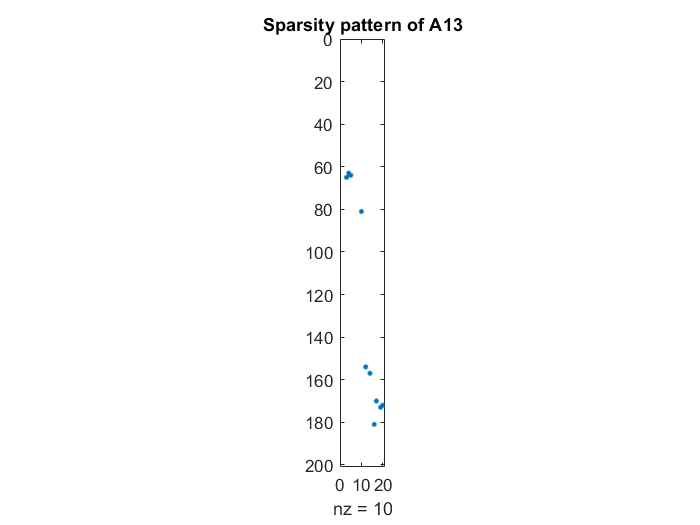
\includegraphics[width=\linewidth]{A13.png}
    \caption{}
    \label{fig:a}
    \vspace{4ex}
  \end{subfigure}%%
  \begin{subfigure}[b]{0.5\linewidth}
    \centering
    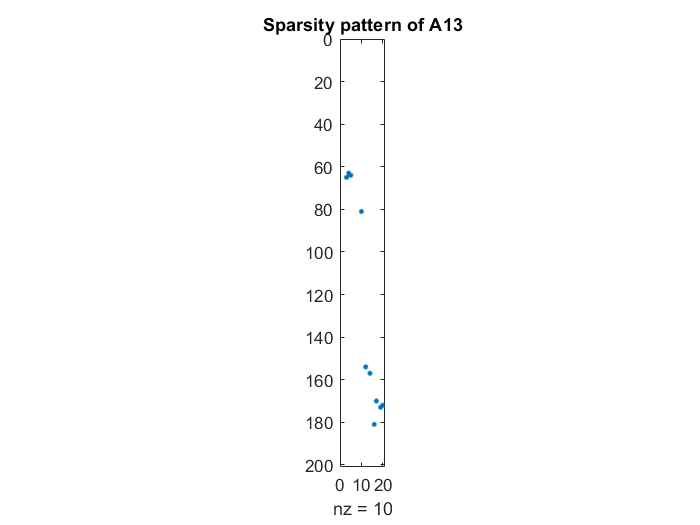
\includegraphics[width=\linewidth]{A13.png}
    \caption{}
    \label{fig:b}
    \vspace{4ex}
  \end{subfigure}
  \begin{subfigure}[b]{0.5\linewidth}
    \centering
    \includegraphics[width=\linewidth]{U11.png}
    \caption{}
    \label{fig:c}
    \vspace{4ex}
  \end{subfigure}%%
  \begin{subfigure}[b]{0.5\linewidth}
    \centering
    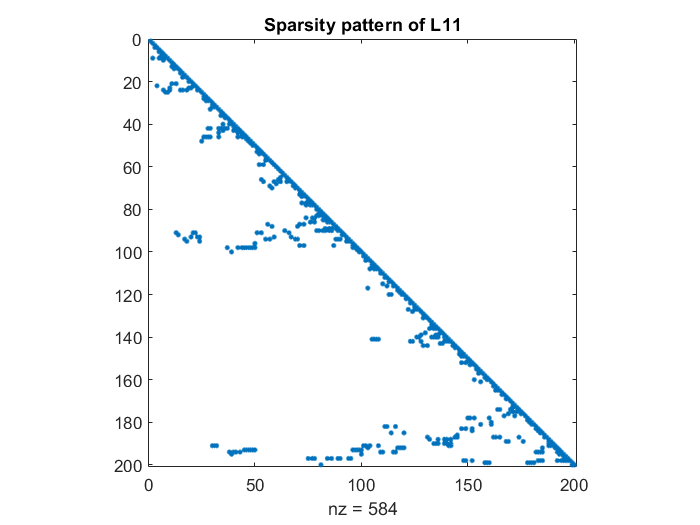
\includegraphics[width=\linewidth]{L11.png}
    \caption{}
    \label{fig:d}
    \vspace{4ex}
  \end{subfigure}
  \caption{}
  \label{fig}
\end{figure}


\begin{figure}[H]
  \begin{subfigure}[b]{0.5\linewidth}
    \centering
    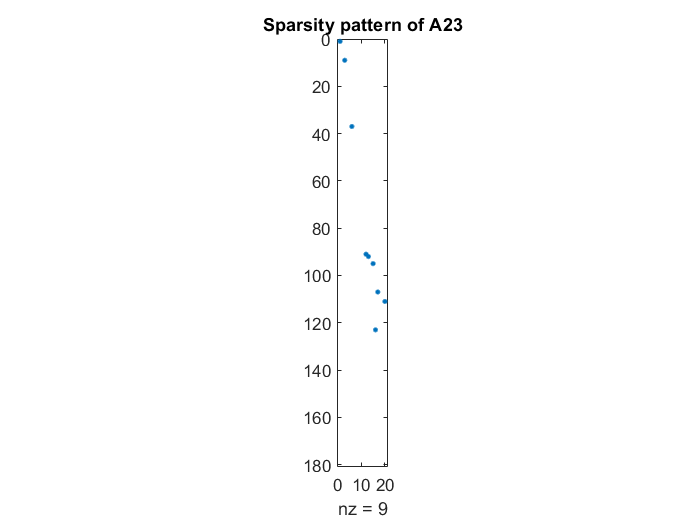
\includegraphics[width=\linewidth]{A23.png}
    \caption{}
    \label{fig1:a}
    \vspace{4ex}
  \end{subfigure}%%
  \begin{subfigure}[b]{0.5\linewidth}
    \centering
    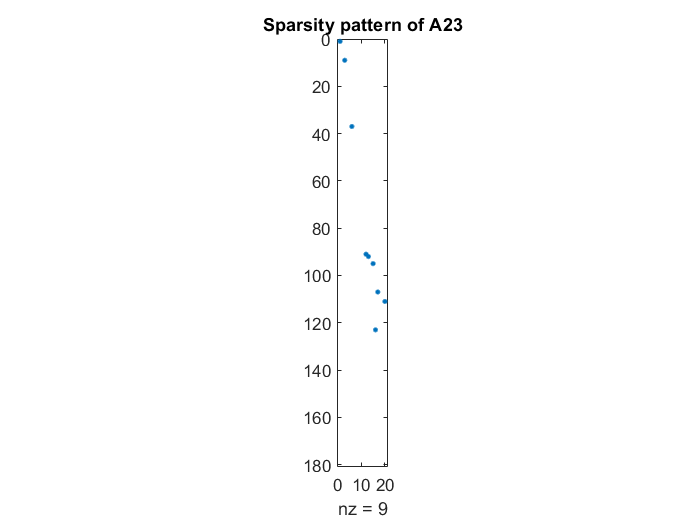
\includegraphics[width=\linewidth]{A23.png}
    \caption{}
    \label{fig1:b}
    \vspace{4ex}
  \end{subfigure}
  \begin{subfigure}[b]{0.5\linewidth}
    \centering
    \includegraphics[width=\linewidth]{U22.png}
    \caption{}
    \label{fig1:c}
    \vspace{4ex}
  \end{subfigure}%%
  \begin{subfigure}[b]{0.5\linewidth}
    \centering
    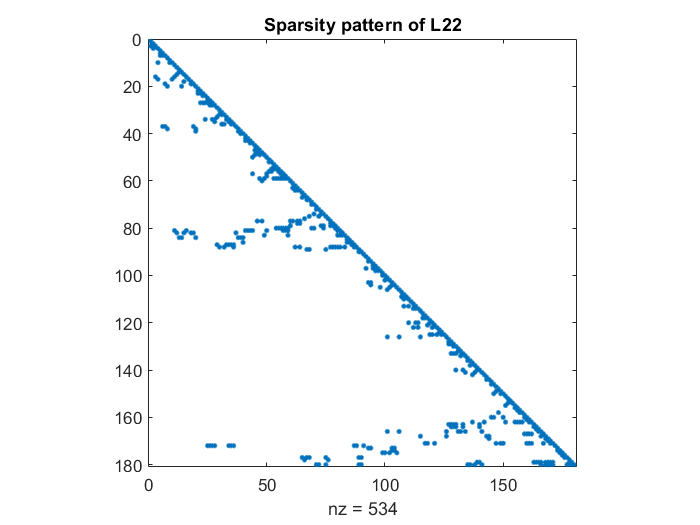
\includegraphics[width=\linewidth]{L22.png}
    \caption{}
    \label{fig1:d}
    \vspace{4ex}
  \end{subfigure}
  \caption{}
  \label{fig1}
\end{figure}


\end{proof}
\end{problem}






\end{document}